\chapter{Preliminary Analysis}

In this section, we provide an in-depth analysis of the EEG data used in the study, focusing on artifact detection and inter-subject variations. These factors are critical to the quality of the EEG signals and directly impact the performance of sleep stage classification models.

\section{Artifact Detection}

EEG data is often contaminated by various artifacts that can interfere with the accurate interpretation of brain activity, particularly in the context of sleep stage classification. This analysis focuses on identifying common types of artifacts, including power line noise, cardiac signal noise, eye movement artifacts, and bad channel noise. These artifacts were identified using diagnostic techniques such as power spectrogram analysis and Independent Component Analysis (ICA), with supporting visualizations provided through graphs and diagnostic plots. \\

In Figure \ref{fig:powerlinenoise}, the power spectrogram for a randomly selected subject clearly shows a distinct spike at 60 Hz, which is indicative of power line noise. This periodic interference is commonly caused by the electrical power grid, which introduces noise at this frequency. Additionally, smaller spikes are observed around multiples of 15 Hz, which can be attributed to cardiac signal noise. This noise results from the electrical activity of the heart, which often contaminates the EEG signal, especially in the low-frequency range. These observations highlight the presence of both power line and cardiac signal artifacts in the EEG data, necessitating appropriate artifact removal techniques for accurate analysis.

\begin{figure}[H]
    \centering
    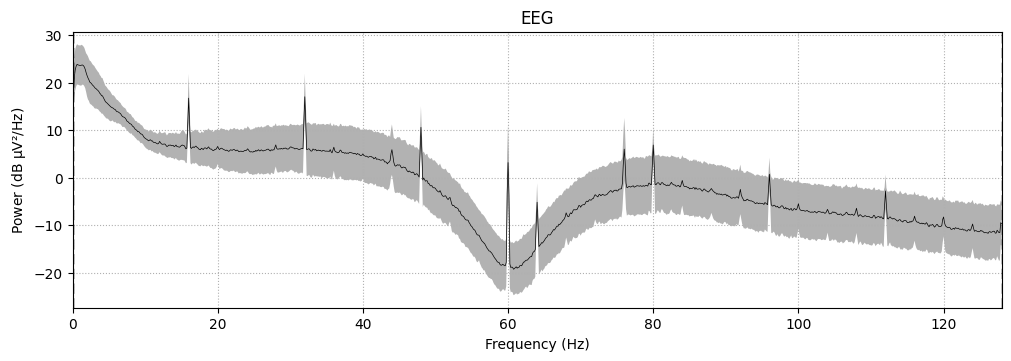
\includegraphics[width=1\linewidth]{Figures/powerlinenoise.png}
    \caption{Power spectrogram showing power line noise and cardiac signal noise of a randomly selected subject.}
    \label{fig:powerlinenoise}
\end{figure} 

In Figure \ref{fig:ica}, the topographic maps for each ICA component of a randomly selected subject are presented. Two components, ICA000 and ICA019, are identified as corresponding to specific artifacts. ICA000 is associated with eye movement artifacts, as evidenced by signal saturation near the eye region. Similarly, ICA019 is linked to a bad channel, with signal saturation localized to a single area. These findings are crucial for identifying and isolating artifacts in the EEG data for further analysis.

\begin{figure}[H]
    \centering
    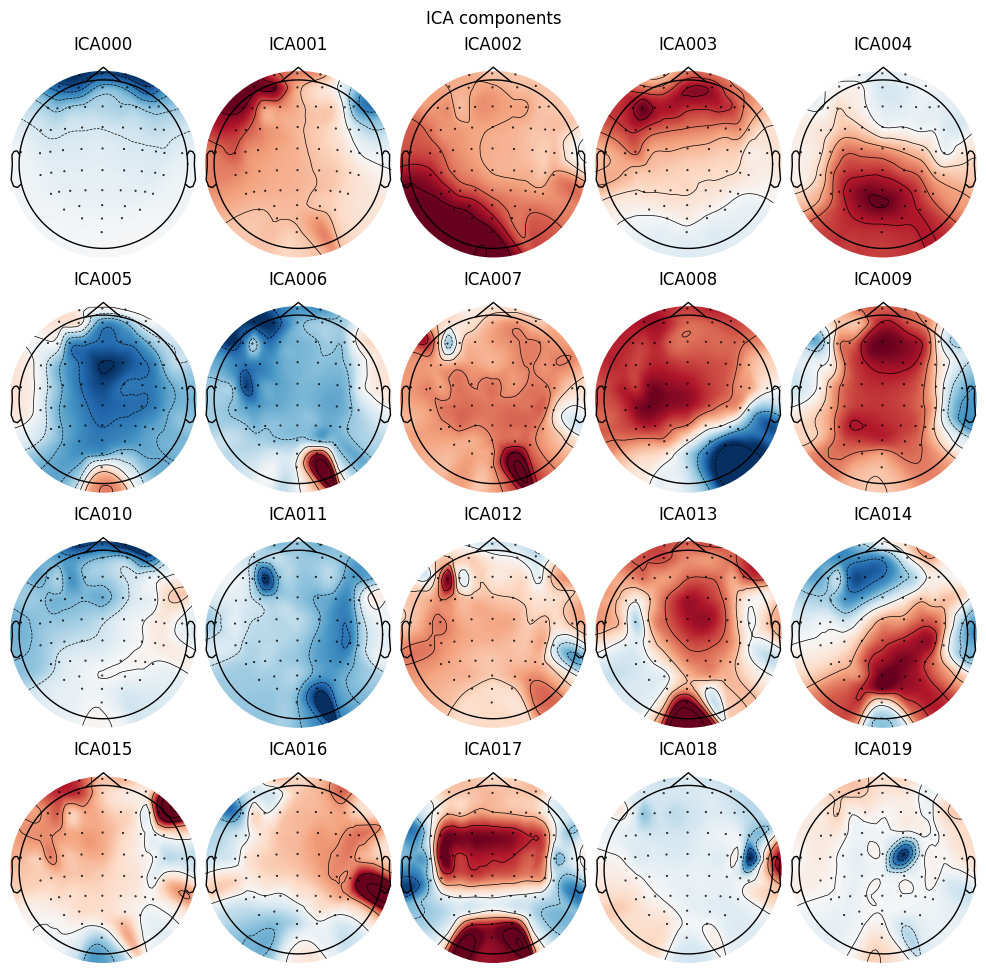
\includegraphics[width=0.6\linewidth]{Figures/ica.png}
    \caption{Topographic maps for ICA components of a randomly selected subject.}
    \label{fig:ica}
\end{figure} 

By eliminating these artifacts, the quality of the data is significantly improved. Hence removal of artifacts through signal preprocessing is essential for ensuring the accuracy and reliability of EEG data in sleep stage classification. 

\section{Inter Subject Variations in EEG}

Inter-subject variations are differences in EEG signals that arise between different individuals. These variations can be attributed to numerous factors, including individual differences in brain structure, electrode placement, and physiological responses during sleep. Inter-subject variability is one of the most significant challenges in EEG-based sleep stage classification, as it can make it difficult for models trained on one subject’s data to generalize effectively to others. \\

Figure \ref{fig:s_power} presents the power spectrograms of three randomly selected subjects for their S3 sleep stage. It is evident that the spectrograms exhibit distinct patterns for each subject, reflecting variations in the EEG signal characteristics. These differences highlight the individual variability in the brain’s electrical activity during sleep, which must be accounted for in analysis and model training to ensure generalization across subjects. \\

Further, Figure \ref{fig:connectivity} presents the connectivity matrices of EEG electrodes for two randomly selected subjects during the same sleep stage (S3). The matrices reveal noticeable differences in electrode connectivity between the subjects. This variability further emphasizes the need for handle inter-subject differences effectively. Recognizing and addressing such variations is crucial for improving the performance of sleep stage classification models, as it helps ensure that the model generalizes well across diverse data sources. \\ 

By understanding and addressing inter-subject variability in EEG data, the accuracy and reliability of sleep stage classification can be improved, ultimately leading to more effective and personalized analyses.

\begin{figure}[H]
    \centering
    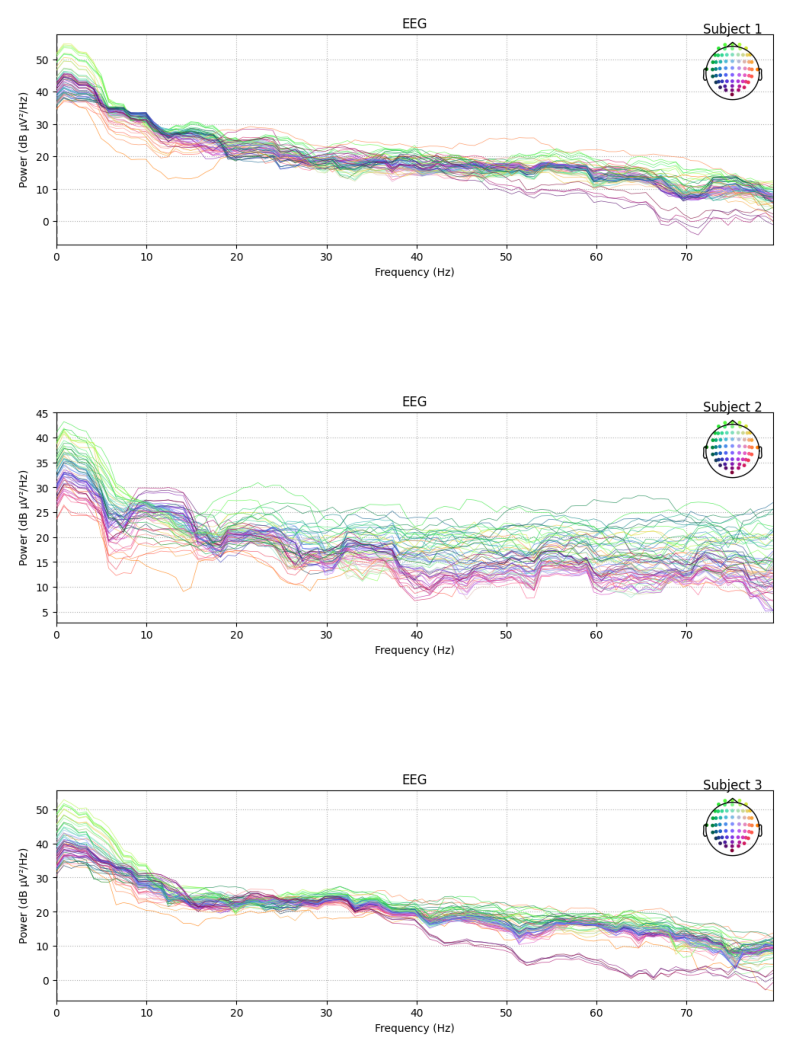
\includegraphics[width=0.65\linewidth]{Figures/s_power.png}
    \caption{Power spectrograms for three randomly selected subjects showing distinct EEG signal patterns across S3 sleep stage.}
    \label{fig:s_power}
\end{figure}

\begin{figure}[H]
    \centering
    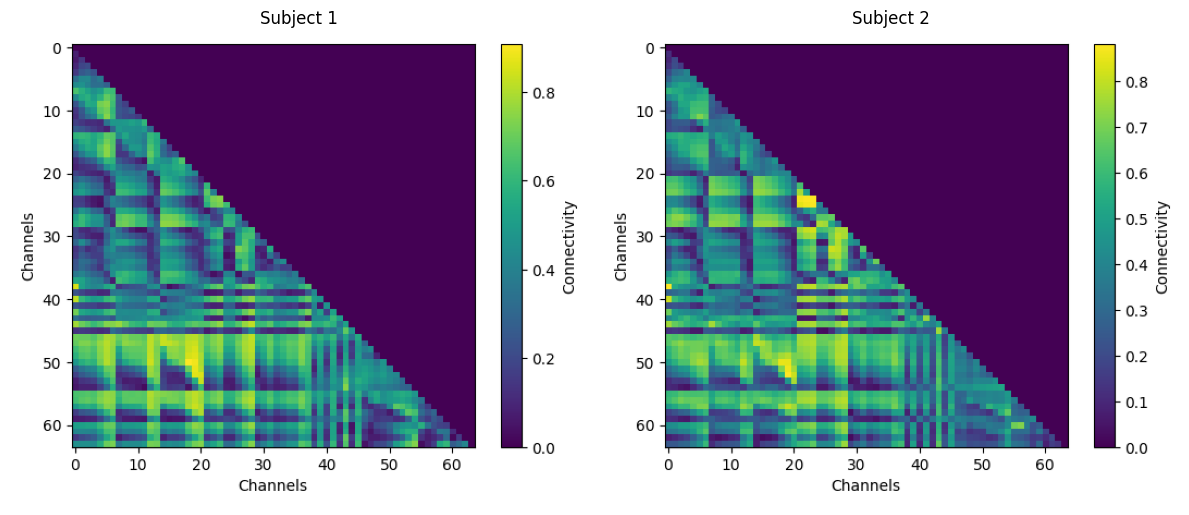
\includegraphics[width=1\linewidth]{Figures/connectivity.png}
    \caption{Connectivity matrices for two randomly selected subjects during the S3 sleep stage.}
    \label{fig:connectivity}
\end{figure}

